% This is the template for submission of abstracts to NetSci 2026 in Boston, USA.
% It is modified from NetSci2024, which was inspired by that of NetSci2016 and that of STATPHSY25.
% The editor of the booklet reserves the right to modify your submission.

% To process this file run LaTeX2e

% ******** DO NOT EDIT ****************
\documentclass[10pt]{article}
% \usepackage{mathptmx}
\usepackage[letterpaper,margin=20mm]{geometry}
\usepackage{graphicx}
\usepackage{lmodern}
\renewcommand{\familydefault}{\sfdefault}
\pagestyle{empty}
\setlength{\parskip}{0.25\baselineskip}
\renewcommand{\title}[1]{{\noindent\large\bfseries#1\medskip\\}}
\renewcommand{\author}[2]{{\noindent #1 \medskip\\ \noindent \small #2 \medskip\\}}
% *************************************

\begin{document}

% ********** USER DEFINED *************

\title{Rising Dispersion in Country-Level Academic Mobility Rankings from ORCID-Derived Flow Networks}

\author{
Li Yifeng\textsuperscript{1}
}
{
1. University of Trento, Trento, Italy
}

We study whether the global academic mobility system has become more stratified in recent years by constructing country-to-country mobility flow networks from longitudinal affiliation episodes in the ORCID Public Data File (2025 release). 
From ORCID affiliation transitions, we build directed weighted networks where edge weights represent cross-border mobility volume between countries (country codes normalized via ISO 3166-1 mappings). 
To quantify structural position in these mobility networks, we compute country scores using SpringRank, a generative, flow-based ranking method for directed networks. 
We then perform a temporal analysis using centered sliding windows (e.g., 3-year windows centered at each year) to obtain yearly distributions of country SpringRank scores.
To summarize system-level inequality, we track the weighted dispersion (weighted standard deviation) of country scores in each window, using total mobility volume as weights.

Across the observation period (2007--2025), we observe a marked increase in score dispersion beginning around 2020, indicating a widening separation between countries that consistently occupy high-ranked positions in global mobility flows and those that remain peripheral.
Because the dispersion metric aggregates over all countries, it provides a compact view of system-level stratification beyond individual country trajectories.
These findings are consistent with an increasingly uneven mobility landscape, where a smaller set of countries concentrates a growing share of high-rank positions and mobility influence.
Our dataset release and end-to-end pipeline enable independent verification and extension of the analysis.

\bigskip
{\small
\noindent[1] ORCID. \textit{ORCID Public Data File 2025} [dataset]. 2025. doi:10.23640/07243.30375589.\\
\noindent[2] De Bacco C, Power EA, Larremore DB, Moore C. A physical model for efficient ranking in networks. \textit{Sci Adv}. 2018;4:eaar8260. doi:10.1126/sciadv.aar8260.\\
\noindent[3] Li Y. \textit{ORCID-derived Academic Mobility Networks} [dataset]. Zenodo; 2025. doi:10.5281/zenodo.17983291.\\
\noindent[4] Datasets Project (DataHub). \textit{country-list (ISO 3166-1)} [dataset]. datahub.io/core/country-list. Accessed 2025-12-19.\\
\noindent[5] Li Y. \textit{osr-examples: Analysis pipelines and figures for ORCID-derived academic mobility networks} [computer software]. GitHub. Accessed 2025-12-19.
}

\begin{figure}[!h]
  \centering
  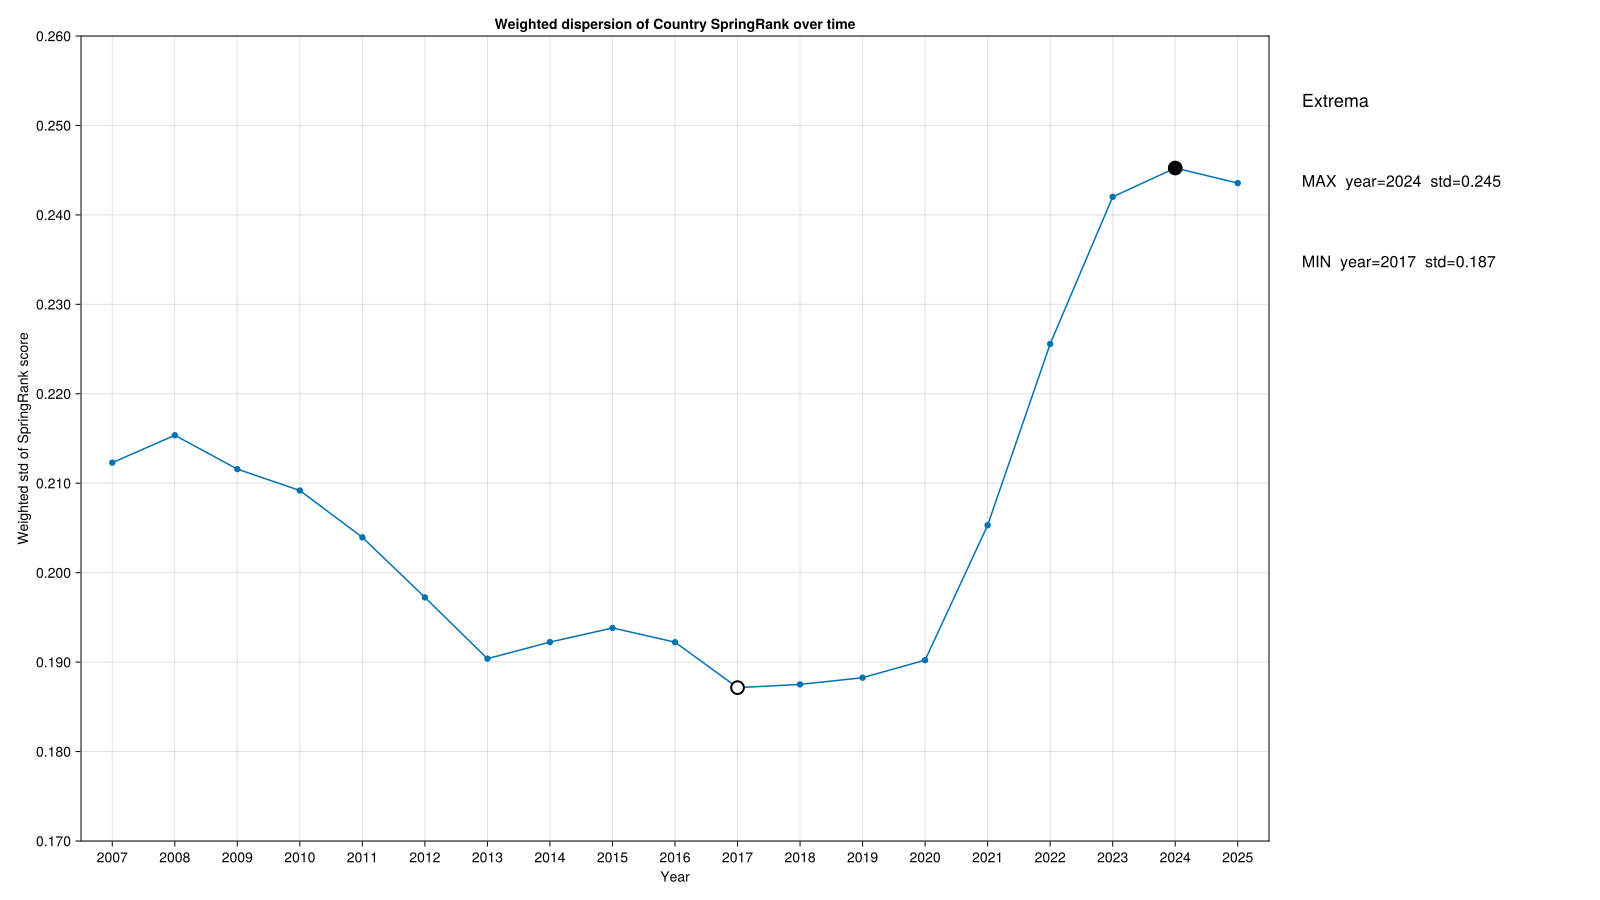
\includegraphics[width=0.78\textwidth]{../figure/fig2_country_springrank_dispersion_weighted_std.pdf}
  \caption{\textbf{Rising dispersion in country SpringRank scores.} Weighted standard deviation of country SpringRank scores computed on centered sliding windows of ORCID-derived mobility flow networks. Weights are proportional to total mobility volume in each window. A sustained rise after 2020 indicates increasing stratification in the country-level mobility ranking distribution.}
\end{figure}



% *************************************
\end{document}